% %\subsection{Perception Component Performance}
% We evaluated the segmentation backbone on the LaRS validation split. SegFormer achieves an obstacle recall of 96.51\%, substantially outperforming a DeepLab baseline (79.83\% recall) at comparable cost. This high recall is critical for safety-oriented ASV operation, where missed low-profile hazards such as buoys, swimmers, or floating debris can be catastrophic. For monocular depth, the evaluation was conducted using the radar data from the WaterScenes dataset, where the Base model provides a mean absolute error (MAE) of 4.04 m within the critical 0–20 m range. While the Large variant offers lower error (3.22\,m), its high latency is prohibitive for real-time edge navigation.

% %\subsection{End-to-End Pipeline and Efficiency}
% The integrated pipeline was evaluated on real-world maritime sequences from the MODD\cite{Kristan2015} dataset. As demonstrated by the qualitative results in Fig.~\ref{fig:pipeline_examples}, the system reliably distinguishes between stable and escalating risk states. The system maintains these transitions with high temporal stability; the warning distribution (62\% SAFE, 33\% CAUTION, 5\% IMMEDIATE) remained consistent with the obstacle dynamics, with no observed warning-level flicker.

% In terms of computational efficiency, the total system latency is 73.0 ms, sustaining approximately 13.7 FPS on a NVIDIA RTX 4060 GPU. Depth estimation is the primary bottleneck (38.7 ms), followed by segmentation (26.9 ms) and risk reasoning (7.4 ms). 
% % The system sustains 13.7 FPS (73.0 ms latency) on an RTX 4060 GPU. Latency is dominated by depth estimation (38.7 ms) and segmentation (26.9 ms), with minimal overhead for risk reasoning (7.4 ms).
% This low overhead for risk reasoning leaves significant headroom for future integration of higher-rate sensors or more complex fusion logic.

% \begin{figure}[t]
%     \centering
%     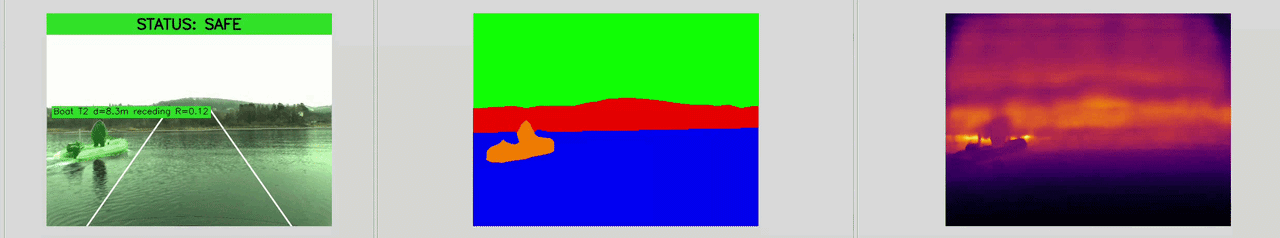
\includegraphics[width=\linewidth]{images/example1_safe.png}\\[2pt]
%     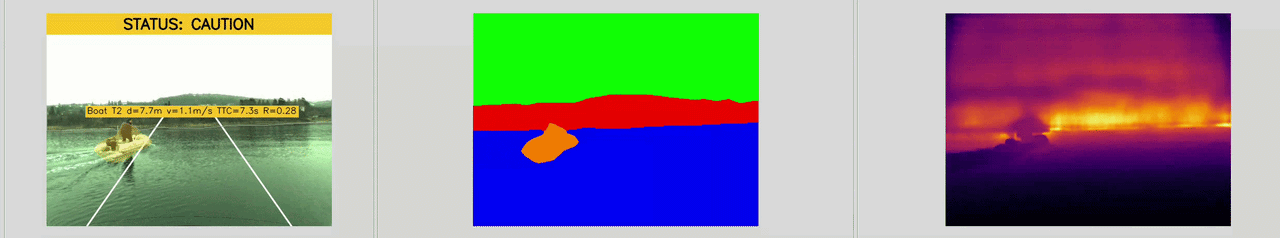
\includegraphics[width=\linewidth]{images/example1_caution.png}
%     \caption{Qualitative evaluation on a MODD sequence. As the tracked boat enters the virtual collision corridor, the system transitions from SAFE (top) to CAUTION (bottom). Each row shows the annotated RGB frame (left), semantic segmentation (center), and monocular depth map (right).\vspace{-4mm}}
%     \label{fig:pipeline_examples}
% \end{figure}

\subsection{Semantic Segmentation}
We evaluate the segmentation backbone against a DeepLab baseline on the LaRS~\cite{zust2023larsdiversepanopticmaritime} validation split, weighting obstacle recall and inference latency over aggregate pixel accuracy, in line with the safety-oriented evaluation stated in Section I. Table~\ref{tab:seg_compare} summarizes the comparison: SegFormer reaches 96.51\% obstacle recall, nearly 17 percentage points above DeepLab's 79.83\%, so far fewer hazardous obstacles go undetected. The gain comes at a latency cost: 29.74\,ms per frame against 15.44\,ms for DeepLab, though both remain compatible with real-time operation at typical ASV speeds.

\begin{table}[t]
\centering
\caption{Comparison of DeepLab and SegFormer on the LaRS validation set.}
\label{tab:seg_compare}
\begin{tabular}{lcc}
\hline
Metric & DeepLab & SegFormer \\
\hline
Obstacle Recall & 0.7983 & 0.9651 \\
Obstacle Precision & 0.9648 & 0.9737 \\
Avg.\ Latency (ms) & 15.44 & 29.74 \\
\hline
\end{tabular}
\end{table}

Per-class IoU on a held-out set of 198 test images (Table~\ref{tab:per_class_iou}) shows where this recall advantage comes from and where the model still struggles. Dominant background classes are segmented almost perfectly, 0.9703 for Water and 0.9618 for Sky, and large static obstacles reach 0.9056. Small or infrequent hazard classes fare far worse: Buoy scores 0.2036, Swimmer 0.4254, and Animal (0.0068) and Float (0.0000) are essentially unrecovered, pulling the class-averaged mIoU down to 0.4823 despite the strong recall figure above. The gap reflects severe class imbalance in LaRS together with the small spatial footprint and appearance variability of these objects, and it matters less for our purposes than it would elsewhere, since the downstream risk model depends on obstacle presence and a conservative depth percentile rather than a pixel-accurate boundary.

\begin{table}[t]
\centering
\caption{Per-class IoU on the segmentation test set (SegFormer).}
\label{tab:per_class_iou}
\begin{tabular}{lc}
\hline
Class & IoU \\
\hline
Static Obstacle & 0.9056 \\
Water & 0.9703 \\
Sky & 0.9618 \\
Boat & 0.6230 \\
Buoy & 0.2036 \\
Swimmer & 0.4254 \\
Animal & 0.0068 \\
Float & 0.0000 \\
Other & 0.2442 \\
\hline
mIoU & 0.4823 \\
\hline
\end{tabular}
\end{table}

Figure~\ref{fig:seg_qual} contrasts DeepLab and SegFormer predictions on a representative frame. Both recover the dominant sky and water regions, but DeepLab fragments the thin obstacle band near the waterline, while SegFormer preserves a more continuous region that matches the ground-truth overlay more closely, consistent with its higher measured recall.

\begin{figure*}[t]
\centering
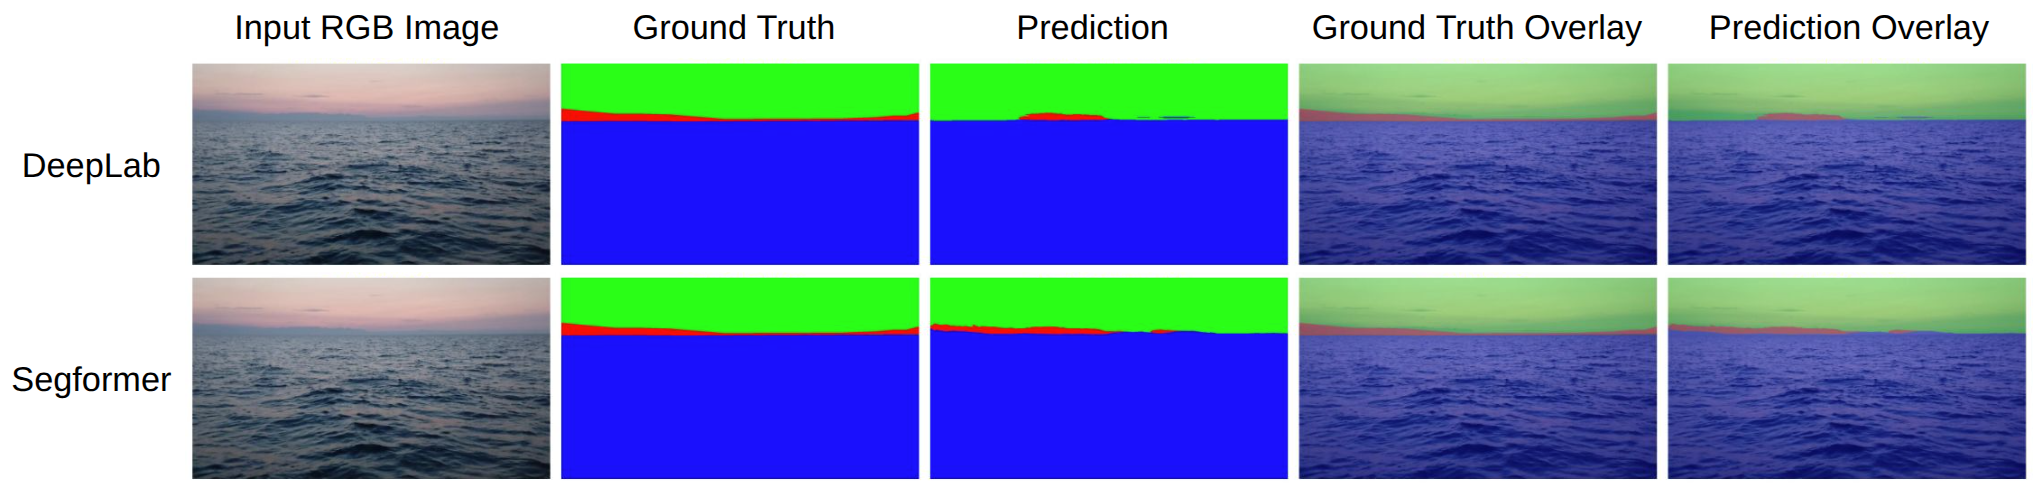
\includegraphics[width=\textwidth]{images/deeplabVSsegformer.png}
\caption{Qualitative comparison of DeepLab and SegFormer on a representative maritime frame.}
\label{fig:seg_qual}
\end{figure*}

\subsection{Monocular Depth Estimation}
We benchmark three variants of the Metric-Outdoor Depth Anything V2 model, small, base, and large, against 33,648 radar-aligned points drawn from the WaterScenes~\cite{yao2024waterscenesmultitask4dradarcamera} sample subset, applying the calibration described in Section III-B. Table~\ref{tab:depth_compare} reports accuracy within the 0--20\,m range that matters most for collision warning. The large model is the most accurate, MAE 3.215\,m with an Est/GT ratio of 1.008 (near-metric scale), but also the slowest at 0.710\,s per image; the small model is fastest (0.149\,s) but least accurate (MAE 4.434\,m). We deploy the base variant in the pipeline as a middle ground (MAE 4.039\,m at 0.279\,s per image): the large model's latency is incompatible with real-time navigation, and the small model's error is too high for reliable collision warning.

\begin{table}[t]
\centering
\caption{Depth model comparison within 0--20\,m.}
\label{tab:depth_compare}
\begin{tabular}{lccc}
\hline
Model & MAE (m) & RMSE (m) & Est/GT \\
\hline
Small & 4.434 & 5.719 & 0.787 \\
Base & 4.039 & 5.363 & 0.887 \\
Large & 3.215 & 4.471 & 1.008 \\
\hline
\end{tabular}
\end{table}

Even after calibration, accuracy degrades beyond 20\,m: median inter-frame depth variation is 0.28\,m on our evaluation sequences, and predictions saturate near the model's built-in depth ceiling of approximately 80\,m, which the calibration factor $s_{cal}=0.4$ maps down to roughly 32\,m. Figure~\ref{fig:depth_qual} shows this behavior directly: the estimated-versus-ground-truth scatter clusters tightly along the diagonal at short range but drifts and flattens as distance grows toward the saturation point.

\begin{figure}[t]
\centering
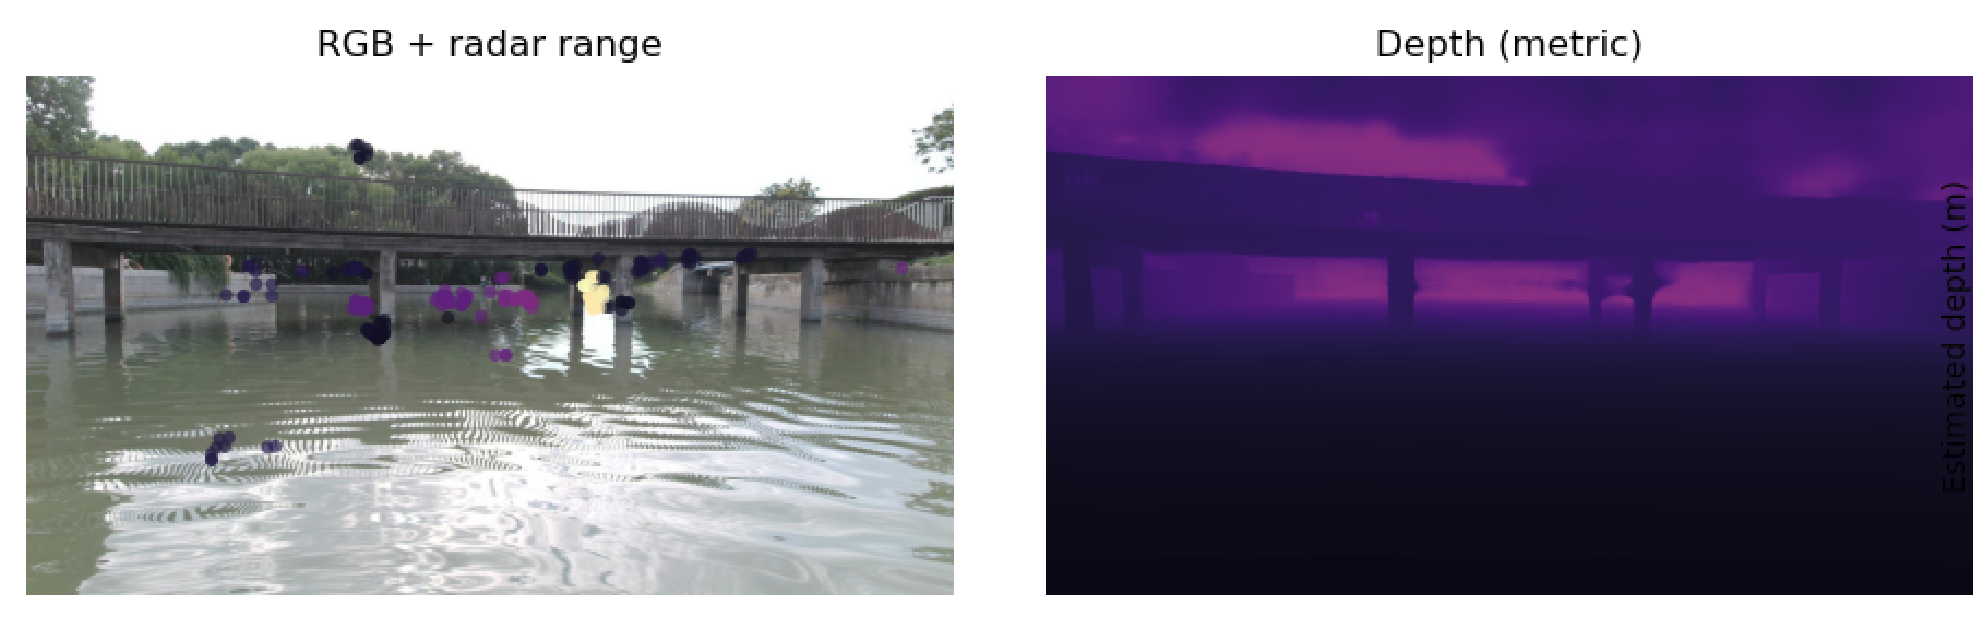
\includegraphics[width=\linewidth]{images/depth_estvsgt_1.png}\\[2pt]
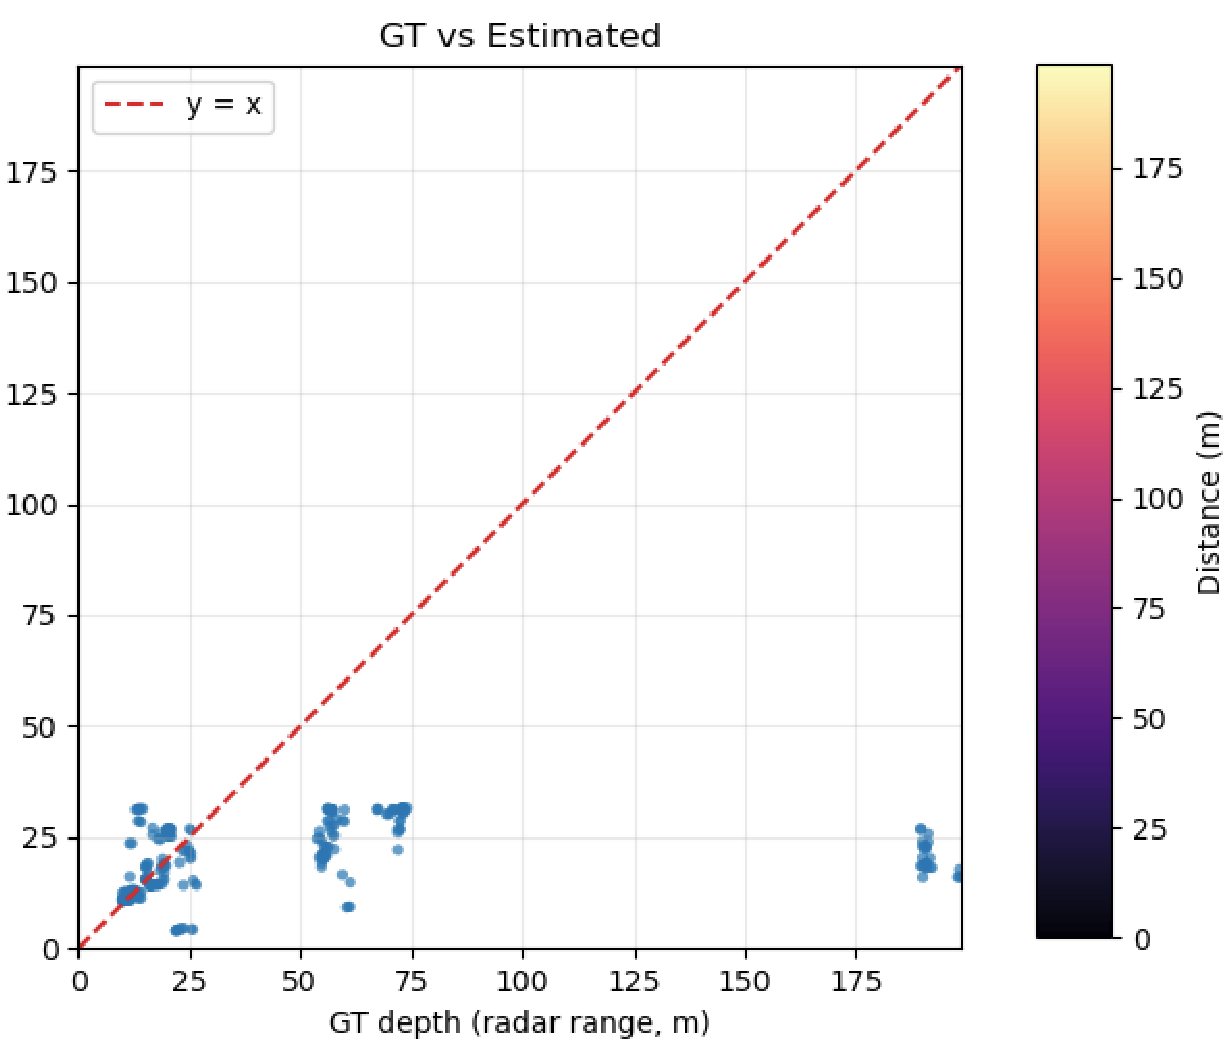
\includegraphics[width=0.8\linewidth]{images/depth_estvsgt_2.png}
\caption{Monocular depth evaluation against radar ground truth. Top: input RGB with projected radar range points (left) and the corresponding calibrated depth map (right). Bottom: estimated depth versus radar ground truth across the evaluation set; the dashed line marks perfect agreement.}
\label{fig:depth_qual}
\end{figure}

\subsection{End-to-End Pipeline Performance}
We assess end-to-end viability on real-world sequences from the MODD~\cite{Kristan2015} dataset, running the segmentation, depth, tracking, and risk-model stages together as a single pipeline. Across 419 tested frames containing tracked obstacles, the system reports 62\% SAFE, 33\% CAUTION, and 5\% IMMEDIATE, with no observed flicker between adjacent frames. The Kalman-filtered depth and velocity, the EMA-smoothed lateral offset, and the hysteresis thresholds described in Section III jointly suppress the frame-to-frame noise that would otherwise destabilize the warning signal. Figure~\ref{fig:pipeline_qual} shows two representative sequences: in the first, a tracked boat closes distance and its closing velocity rises, driving the system from SAFE through CAUTION to IMMEDIATE WARNING; in the second, a buoy produces a SAFE-to-CAUTION transition as the ASV approaches, with the overlaid track ID, distance estimate, and risk score updating consistently across frames in both cases.

\begin{figure}[t]
\centering
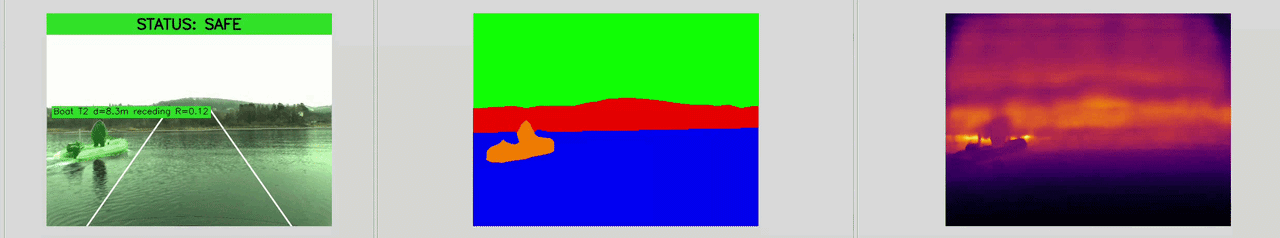
\includegraphics[width=\linewidth]{images/example1_safe.png}\\[2pt]
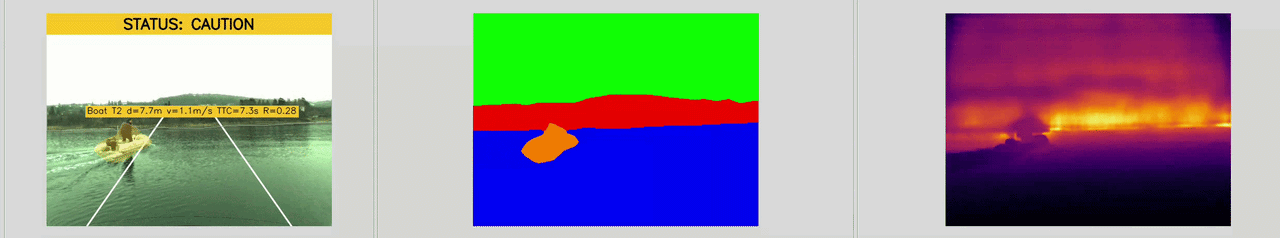
\includegraphics[width=\linewidth]{images/example1_caution.png}\\[2pt]
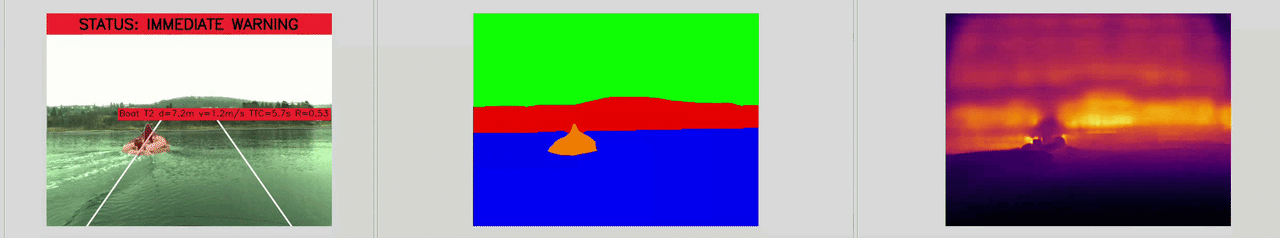
\includegraphics[width=\linewidth]{images/example1_warning.png}\\[2pt]
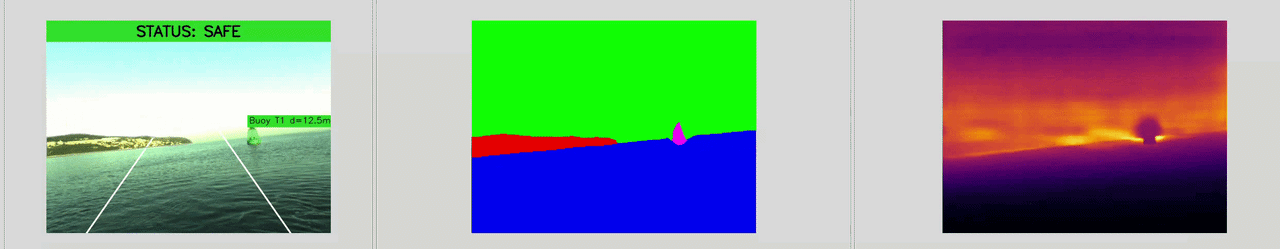
\includegraphics[width=\linewidth]{images/example2_safe.png}\\[2pt]
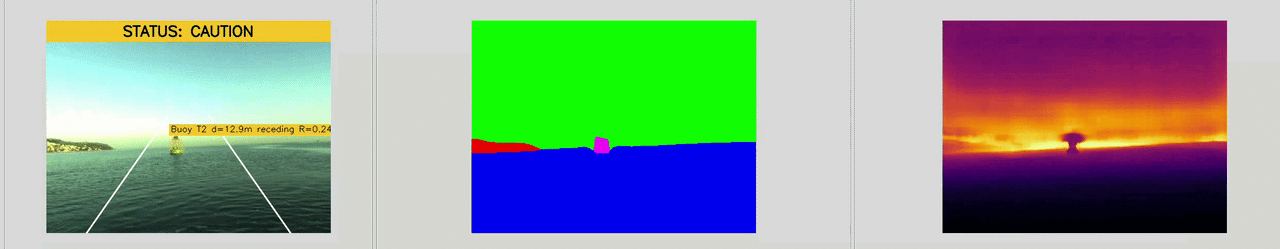
\includegraphics[width=\linewidth]{images/example2_caution.png}
\caption{Qualitative evaluation on two MODD sequences. Rows 1--3: a tracked boat closes distance and the system escalates from SAFE to CAUTION to IMMEDIATE WARNING. Rows 4--5: a tracked buoy produces a SAFE-to-CAUTION transition as the ASV approaches. Each row shows the annotated RGB frame (left), semantic segmentation (center), and monocular depth map (right).}
\label{fig:pipeline_qual}
\end{figure}

Table~\ref{tab:latency} breaks down the average per-frame latency of the full pipeline on an NVIDIA RTX 4060 GPU. Depth estimation dominates the budget at 38.7\,ms (53\% of the total), followed by segmentation at 26.9\,ms; the fusion and risk-reasoning stage adds only 7.4\,ms. The resulting total of 73.0\,ms sustains roughly 13.7\,FPS, sufficient for real-time collision warning at typical inland-vessel speeds and leaving headroom for future additions such as higher-rate sensors or more elaborate fusion logic.

\begin{table}[t]
\centering
\caption{Average inference latency of the end-to-end pipeline.}
\label{tab:latency}
\begin{tabular}{lc}
\hline
Pipeline Component & Avg.\ Latency (ms) \\
\hline
Semantic Segmentation (SegFormer) & 26.9 \\
Depth Estimation (Depth Anything V2) & 38.7 \\
Temporal Fusion \& Risk Modeling & 7.4 \\
\hline
Total System Latency & 73.0 \\
\hline
\end{tabular}
\end{table}

\subsection{Limitations}
Several limitations affect these results. Segmentation accuracy on rare hazard classes remains low (Buoy 0.2036, Swimmer 0.4254, Animal 0.0068, and Float 0.0000 IoU), so the pipeline depends on obstacle presence and coarse localization rather than fine-grained recognition. Depth calibration saturates beyond roughly 32\,m, which is acceptable for the near-field collision-warning band but leaves longer-range hazards unranged. End-to-end validation is also confined to MODD sequences from a single forward-facing camera; robustness to vessel heave and pitch, extreme lighting, and obstacles outside the camera's field of view has not yet been tested on physical hardware.
